
%% bare_conf.tex
%% V1.4b
%% 2015/08/26
%% by Michael Shell
%% See:
%% http://www.michaelshell.org/
%% for current contact information.
%%
%% This is a skeleton file demonstrating the use of IEEEtran.cls
%% (requires IEEEtran.cls version 1.8b or later) with an IEEE
%% conference paper.
%%
%% Support sites:
%% http://www.michaelshell.org/tex/ieeetran/
%% http://www.ctan.org/pkg/ieeetran
%% and
%% http://www.ieee.org/

%%*************************************************************************
%% Legal Notice:
%% This code is offered as-is without any warranty either expressed or
%% implied; without even the implied warranty of MERCHANTABILITY or
%% FITNESS FOR A PARTICULAR PURPOSE! 
%% User assumes all risk.
%% In no event shall the IEEE or any contributor to this code be liable for
%% any damages or losses, including, but not limited to, incidental,
%% consequential, or any other damages, resulting from the use or misuse
%% of any information contained here.
%%
%% All comments are the opinions of their respective authors and are not
%% necessarily endorsed by the IEEE.
%%
%% This work is distributed under the LaTeX Project Public License (LPPL)
%% ( http://www.latex-project.org/ ) version 1.3, and may be freely used,
%% distributed and modified. A copy of the LPPL, version 1.3, is included
%% in the base LaTeX documentation of all distributions of LaTeX released
%% 2003/12/01 or later.
%% Retain all contribution notices and credits.
%% ** Modified files should be clearly indicated as such, including  **
%% ** renaming them and changing author support contact information. **
%%*************************************************************************


% *** Authors should verify (and, if needed, correct) their LaTeX system  ***
% *** with the testflow diagnostic prior to trusting their LaTeX platform ***
% *** with production work. The IEEE's font choices and paper sizes can   ***
% *** trigger bugs that do not appear when using other class files.       ***                          ***
% The testflow support page is at:
% http://www.michaelshell.org/tex/testflow/



\documentclass[conference]{IEEEtran}
% Some Computer Society conferences also require the compsoc mode option,
% but others use the standard conference format.
%
% If IEEEtran.cls has not been installed into the LaTeX system files,
% manually specify the path to it like:
% \documentclass[conference]{../sty/IEEEtran}





% Some very useful LaTeX packages include:
% (uncomment the ones you want to load)


% *** MISC UTILITY PACKAGES ***
%
%\usepackage{ifpdf}
% Heiko Oberdiek's ifpdf.sty is very useful if you need conditional
% compilation based on whether the output is pdf or dvi.
% usage:
% \ifpdf
%   % pdf code
% \else
%   % dvi code
% \fi
% The latest version of ifpdf.sty can be obtained from:
% http://www.ctan.org/pkg/ifpdf
% Also, note that IEEEtran.cls V1.7 and later provides a builtin
% \ifCLASSINFOpdf conditional that works the same way.
% When switching from latex to pdflatex and vice-versa, the compiler may
% have to be run twice to clear warning/error messages.






% *** CITATION PACKAGES ***
%
%\usepackage{cite}
% cite.sty was written by Donald Arseneau
% V1.6 and later of IEEEtran pre-defines the format of the cite.sty package
% \cite{} output to follow that of the IEEE. Loading the cite package will
% result in citation numbers being automatically sorted and properly
% "compressed/ranged". e.g., [1], [9], [2], [7], [5], [6] without using
% cite.sty will become [1], [2], [5]--[7], [9] using cite.sty. cite.sty's
% \cite will automatically add leading space, if needed. Use cite.sty's
% noadjust option (cite.sty V3.8 and later) if you want to turn this off
% such as if a citation ever needs to be enclosed in parenthesis.
% cite.sty is already installed on most LaTeX systems. Be sure and use
% version 5.0 (2009-03-20) and later if using hyperref.sty.
% The latest version can be obtained at:
% http://www.ctan.org/pkg/cite
% The documentation is contained in the cite.sty file itself.

\usepackage{graphicx}


% *** GRAPHICS RELATED PACKAGES ***
%
%\ifCLASSINFOpdf
  %\usepackage[pdftex]{graphicx}
  % declare the path(s) where your graphic files are
  % \graphicspath{{../pdf/}{../jpeg/}}
  % and their extensions so you won't have to specify these with
  % every instance of \includegraphics
  % \DeclareGraphicsExtensions{.pdf,.jpeg,.png}
%\else
  % or other class option (dvipsone, dvipdf, if not using dvips). graphicx
  % will default to the driver specified in the system graphics.cfg if no
  % driver is specified.
  % \usepackage[dvips]{graphicx}
  % declare the path(s) where your graphic files are
  % \graphicspath{{../eps/}}
  % and their extensions so you won't have to specify these with
  % every instance of \includegraphics
  % \DeclareGraphicsExtensions{.eps}
%\fi
% graphicx was written by David Carlisle and Sebastian Rahtz. It is
% required if you want graphics, photos, etc. graphicx.sty is already
% installed on most LaTeX systems. The latest version and documentation
% can be obtained at: 
% http://www.ctan.org/pkg/graphicx
% Another good source of documentation is "Using Imported Graphics in
% LaTeX2e" by Keith Reckdahl which can be found at:
% http://www.ctan.org/pkg/epslatex
%
% latex, and pdflatex in dvi mode, support graphics in encapsulated
% postscript (.eps) format. pdflatex in pdf mode supports graphics
% in .pdf, .jpeg, .png and .mps (metapost) formats. Users should ensure
% that all non-photo figures use a vector format (.eps, .pdf, .mps) and
% not a bitmapped formats (.jpeg, .png). The IEEE frowns on bitmapped formats
% which can result in "jaggedy"/blurry rendering of lines and letters as
% well as large increases in file sizes.
%
% You can find documentation about the pdfTeX application at:
% http://www.tug.org/applications/pdftex





% *** MATH PACKAGES ***
%
\usepackage{amsmath}
% A popular package from the American Mathematical Society that provides
% many useful and powerful commands for dealing with mathematics.
%
% Note that the amsmath package sets \interdisplaylinepenalty to 10000
% thus preventing page breaks from occurring within multiline equations. Use:
%\interdisplaylinepenalty=2500
% after loading amsmath to restore such page breaks as IEEEtran.cls normally
% does. amsmath.sty is already installed on most LaTeX systems. The latest
% version and documentation can be obtained at:
% http://www.ctan.org/pkg/amsmath


\usepackage{mathrsfs}



% *** SPECIALIZED LIST PACKAGES ***
%
%\usepackage{algorithmic}
% algorithmic.sty was written by Peter Williams and Rogerio Brito.
% This package provides an algorithmic environment fo describing algorithms.
% You can use the algorithmic environment in-text or within a figure
% environment to provide for a floating algorithm. Do NOT use the algorithm
% floating environment provided by algorithm.sty (by the same authors) or
% algorithm2e.sty (by Christophe Fiorio) as the IEEE does not use dedicated
% algorithm float types and packages that provide these will not provide
% correct IEEE style captions. The latest version and documentation of
% algorithmic.sty can be obtained at:
% http://www.ctan.org/pkg/algorithms
% Also of interest may be the (relatively newer and more customizable)
% algorithmicx.sty package by Szasz Janos:
% http://www.ctan.org/pkg/algorithmicx




% *** ALIGNMENT PACKAGES ***
%
%\usepackage{array}
% Frank Mittelbach's and David Carlisle's array.sty patches and improves
% the standard LaTeX2e array and tabular environments to provide better
% appearance and additional user controls. As the default LaTeX2e table
% generation code is lacking to the point of almost being broken with
% respect to the quality of the end results, all users are strongly
% advised to use an enhanced (at the very least that provided by array.sty)
% set of table tools. array.sty is already installed on most systems. The
% latest version and documentation can be obtained at:
% http://www.ctan.org/pkg/array


% IEEEtran contains the IEEEeqnarray family of commands that can be used to
% generate multiline equations as well as matrices, tables, etc., of high
% quality.




% *** SUBFIGURE PACKAGES ***
%\ifCLASSOPTIONcompsoc
%  \usepackage[caption=false,font=normalsize,labelfont=sf,textfont=sf]{subfig}
%\else
%  \usepackage[caption=false,font=footnotesize]{subfig}
%\fi
% subfig.sty, written by Steven Douglas Cochran, is the modern replacement
% for subfigure.sty, the latter of which is no longer maintained and is
% incompatible with some LaTeX packages including fixltx2e. However,
% subfig.sty requires and automatically loads Axel Sommerfeldt's caption.sty
% which will override IEEEtran.cls' handling of captions and this will result
% in non-IEEE style figure/table captions. To prevent this problem, be sure
% and invoke subfig.sty's "caption=false" package option (available since
% subfig.sty version 1.3, 2005/06/28) as this is will preserve IEEEtran.cls
% handling of captions.
% Note that the Computer Society format requires a larger sans serif font
% than the serif footnote size font used in traditional IEEE formatting
% and thus the need to invoke different subfig.sty package options depending
% on whether compsoc mode has been enabled.
%
% The latest version and documentation of subfig.sty can be obtained at:
% http://www.ctan.org/pkg/subfig




% *** FLOAT PACKAGES ***
%
%\usepackage{fixltx2e}
% fixltx2e, the successor to the earlier fix2col.sty, was written by
% Frank Mittelbach and David Carlisle. This package corrects a few problems
% in the LaTeX2e kernel, the most notable of which is that in current
% LaTeX2e releases, the ordering of single and double column floats is not
% guaranteed to be preserved. Thus, an unpatched LaTeX2e can allow a
% single column figure to be placed prior to an earlier double column
% figure.
% Be aware that LaTeX2e kernels dated 2015 and later have fixltx2e.sty's
% corrections already built into the system in which case a warning will
% be issued if an attempt is made to load fixltx2e.sty as it is no longer
% needed.
% The latest version and documentation can be found at:
% http://www.ctan.org/pkg/fixltx2e


%\usepackage{stfloats}
% stfloats.sty was written by Sigitas Tolusis. This package gives LaTeX2e
% the ability to do double column floats at the bottom of the page as well
% as the top. (e.g., "\begin{figure*}[!b]" is not normally possible in
% LaTeX2e). It also provides a command:
%\fnbelowfloat
% to enable the placement of footnotes below bottom floats (the standard
% LaTeX2e kernel puts them above bottom floats). This is an invasive package
% which rewrites many portions of the LaTeX2e float routines. It may not work
% with other packages that modify the LaTeX2e float routines. The latest
% version and documentation can be obtained at:
% http://www.ctan.org/pkg/stfloats
% Do not use the stfloats baselinefloat ability as the IEEE does not allow
% \baselineskip to stretch. Authors submitting work to the IEEE should note
% that the IEEE rarely uses double column equations and that authors should try
% to avoid such use. Do not be tempted to use the cuted.sty or midfloat.sty
% packages (also by Sigitas Tolusis) as the IEEE does not format its papers in
% such ways.
% Do not attempt to use stfloats with fixltx2e as they are incompatible.
% Instead, use Morten Hogholm'a dblfloatfix which combines the features
% of both fixltx2e and stfloats:
%
% \usepackage{dblfloatfix}
% The latest version can be found at:
% http://www.ctan.org/pkg/dblfloatfix




% *** PDF, URL AND HYPERLINK PACKAGES ***
%
%\usepackage{url}
% url.sty was written by Donald Arseneau. It provides better support for
% handling and breaking URLs. url.sty is already installed on most LaTeX
% systems. The latest version and documentation can be obtained at:
% http://www.ctan.org/pkg/url
% Basically, \url{my_url_here}.




% *** Do not adjust lengths that control margins, column widths, etc. ***
% *** Do not use packages that alter fonts (such as pslatex).         ***
% There should be no need to do such things with IEEEtran.cls V1.6 and later.
% (Unless specifically asked to do so by the journal or conference you plan
% to submit to, of course. )

% *** Pseudocode PACKAGES ***
\usepackage{amsmath}
\DeclareMathOperator*{\argmin}{arg\,min}
\DeclareMathOperator*{\argmax}{arg\,max}
\usepackage{amssymb}
\usepackage{mathtools}
\usepackage{algorithm}
\usepackage[options]{algorithm2e}
\usepackage{varwidth}
\usepackage[noend]{algpseudocode}
\makeatletter
\def\BState{\State\hskip-\ALG@thistlm}
\makeatother


\newcommand\NB[1]{$\spadesuit$\footnote{NB: #1}}
\newcommand\RP[1]{$\clubsuit$\footnote{RP: #1}}
% reference package for bibtex

%\usepackage{biblatex}
%\addbibresource{mybibliography.bib}

%\usepackage[
%backend=biber,
%style=numeric,
%sorting=ynt
%]{biblatex}

%\addbibresource{mybibliography.bib}


% correct bad hyphenation here
\hyphenation{op-tical net-works semi-conduc-tor}


\begin{document}
%
% paper title
% Titles are generally capitalized except for words such as a, an, and, as,
% at, but, by, for, in, nor, of, on, or, the, to and up, which are usually
% not capitalized unless they are the first or last word of the title.
% Linebreaks \\ can be used within to get better formatting as desired.
% Do not put math or special symbols in the title.
\title{Using Hidden Markov Models to Improve Autonomous Vehicle Decision Making - Problem Formulation}


% author names and affiliations
% use a multiple column layout for up to three different
% affiliations
\author{\IEEEauthorblockN{Rahul Peddi}
\IEEEauthorblockA{Systems and Information Engineering\\
University of Virginia\\
Charlottesville, Virginia\\
Email: rp3cy@virginia.edu}}

% conference papers do not typically use \thanks and this command
% is locked out in conference mode. If really needed, such as for
% the acknowledgment of grants, issue a \IEEEoverridecommandlockouts
% after \documentclass

% for over three affiliations, or if they all won't fit within the width
% of the page, use this alternative format:
% 
%\author{\IEEEauthorblockN{Michael Shell\IEEEauthorrefmark{1},
%Homer Simpson\IEEEauthorrefmark{2},
%James Kirk\IEEEauthorrefmark{3}, 
%Montgomery Scott\IEEEauthorrefmark{3} and
%Eldon Tyrell\IEEEauthorrefmark{4}}
%\IEEEauthorblockA{\IEEEauthorrefmark{1}School of Electrical and Computer Engineering\\
%Georgia Institute of Technology,
%Atlanta, Georgia 30332--0250\\ Email: see http://www.michaelshell.org/contact.html}
%\IEEEauthorblockA{\IEEEauthorrefmark{2}Twentieth Century Fox, Springfield, USA\\
%Email: homer@thesimpsons.com}
%\IEEEauthorblockA{\IEEEauthorrefmark{3}Starfleet Academy, San Francisco, California 96678-2391\\
%Telephone: (800) 555--1212, Fax: (888) 555--1212}
%\IEEEauthorblockA{\IEEEauthorrefmark{4}Tyrell Inc., 123 Replicant Street, Los Angeles, California 90210--4321}}




% use for special paper notices
%\IEEEspecialpapernotice{(Invited Paper)}




% make the title area
\maketitle

% As a general rule, do not put math, special symbols or citations
% in the abstract
\begin{abstract}
\end{abstract}

% no keywords




% For peer review papers, you can put extra information on the cover
% page as needed:
% \ifCLASSOPTIONpeerreview
% \begin{center} \bfseries EDICS Category: 3-BBND \end{center}
% \fi
%
% For peerreview papers, this IEEEtran command inserts a page break and
% creates the second title. It will be ignored for other modes.
\IEEEpeerreviewmaketitle



\section{Introduction}
% no \IEEEPARstart

%    Over the last few years, semi-autonomous and autonomous vehicles have become increasingly popular, but they have not replaced traditional vehicles entirely just yet. This leads to a hybrid environment; one that features vehicles of all levels of autonomy. Many of these vehicles to be equipped with some form of adaptive cruise control (ACC) or advance driver assistance systems (ADAS), both of which help the driver make safe decisions while operating the vehicle. These types of systems are forms of human-robot interaction. ACC performs actions autonomously and works at the command of a human who determines a target velocity and a safe following distance. ADAS, on the contrary, acts as an information system for human drivers. These systems, however, are limited in their capabilities as they require constant monitoring from the driver and are unable to predict if the driver will enter a dangerous situation in the future. In addition, these systems can fail to guarantee safety in rapidly transitioning environments.
    
    
%    Because these dangerous situations can occur so rapidly \NB{need citation here}, there is a need to increase the ability to guarantee safety when developing new systems \NB{what do you mean with new systems?} for human drivers. This can be done by increasing the ability to predict and adapt to what will happen in the future. A simple depiction of a danger situation is shown in Fig. \ref{fig:hiway}. \NB{figure needs improvements}
 
\NB{In a not far future, multiple vehicles with different level of autonomy will have to coexist and operate safely. Examples of such vehicles include cars, vessels, aerial vehicles. Different level of autonomy are available 1 to 5 for cars, hobby  } 
    
\NB{Semi-autonomous and autonomous vehicles are finding their way in our society rapidly. Although new advancements in sensing and autonomy are increasing safety by assisting drivers with line changing warning and assisted braking, } Over the last few years, semi-autonomous and autonomous vehicles have become increasingly popular, but they have not replaced traditional vehicles entirely just yet. This leads to a hybrid environment; one that features vehicles of all levels of autonomy.
    
    Many of these vehicles are equipped with some form of adaptive cruise control (ACC) or advance driver assistance systems (ADAS), both of which help the driver make safe decisions while operating the vehicle. These types of systems are forms of human-robot interaction. ACC performs actions autonomously and works at the command of a human who determines a target velocity and a safe following distance. ADAS, on the other hand, acts as an information system for human drivers. These systems, however, are limited in their capabilities as they require constant monitoring from the driver and are unable to predict if the driver will enter a dangerous situation in the future. In addition, these systems can fail to guarantee safety in rapidly transitioning environments.
    

\begin{figure}[ht]
    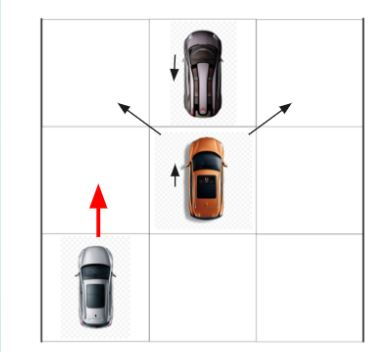
\includegraphics[width=0.5\textwidth]{highwaysit.JPG}
    \caption{A highway: a common situation in which the environment is rapidly changing. The vehicle in the center of the grid is our vehicle, and the vehicle in front is driving much slower, while the vehicle to the right is approaching very rapidly. It would be safe in the instant to pass on the left, but that leaves the possibility that a dangerous situation will occur very soon.}
    \label{fig:hiway}
\end{figure}
    
    In Fig.\ref{fig:hiway}, a  user is driving a vehicle (the vehicle in the center) in a space surrounded by other vehicles. If the driver is unaware of the future risk of performing a certain action, an unsafe situation may arise, resulting in a collision. To resolve this, we are interested in predicting future states of other vehicles, assess risk of collisions given the user's actions, and adapt the system accordingly.This type of work can be approached as a type of Markov Chain, and we leverage Hidden Markov Model (HMM) theory as well, both of which are commonly used models for many cyber-physical systems.
    
     In this work, we aim to provide
    \begin{itemize}
    \item{a prediction method that can effectively and efficiently estimate the future positions of surrounding agents}
    \item{an adaptive framework that determines the adjustment of a user's actions and severity of such adjustment that should be made at any point in time}
    \end{itemize}
  
   Although the proposed approach is applied in the context of autonomous and semi-autonomous vehicles, it is general and applicable to any other CPS. In this case, we see the user as a disturbance or an unintentionally adversarial effect. We monitor the user behavior and intervene if necessary by predicting future states of our system and the surrounding entities (obstacles and other vehicles).    
    
    The rest of this paper is organized as follows: in Section II, we discuss related work, and in Section III, we formally define the problem. The proposed AHMM framework is presented in Section IV. In Section V, we discuss a specific case study, in which our framework is applied to guarantee safety. We demonstrate our results with MATLAB simulations and real-world experiments in Sections VI and VII, respectively. Lastly, we discuss our conclusions and future work in Section VII.

    
% You must have at least 2 lines in the paragraph with the drop letter
% (should never be an issue)

\section{Related Work}

%    This work is tuned a relatively specific situation; one where the host vehicle is driving in the middle lane of a three-lane highway. This was chosen in order to account for a large action space. In this case, there are three possible actions the host vehicle could take, and each of these actions is evaluated for safety. The action space is defined such that it only looks at the immediately adjacent lanes. For example, if the vehicle is in the left lane, the action space consists of forward, and move right. In this case, only those two actions are evaluated for safety at a future time step.
    
    
%    A Hidden Markov Model is a type of Markov Model, where the states are hidden. A Markov Model examines states and transitions to and from these states. An HMM operates on the assumption that we don't directly know what the state is, but we are able to make observations that can tell us valuable information about the current state. Hidden Markov Models have been used for many human-robot interaction applications \cite{li2016modeling}, including but not limited to speech recognition, motion recognition, and biological analyses \cite{yoon2009hidden}.
    
%    In addition to the host vehicle at the center of the road, there are two additional vehicles; one passing on the left lane, and a slowed vehicle ahead in the center lane, as shown in Figure \ref{fig:actionspace}.
    
%    The HMM was performed on the blue vehicle to the left (the purple vehicle is a representation of the estimate), from the perspective of the black vehicle, the host vehicle. The testing was done such that only one vehicle was able to make estimations, but in a truly hybrid environment, multiple vehicles will this technique will improve the ability for multiple vehicles to collaborate.
    
\section{Problem Formulation}
 
In this work we are interested in finding an approach to proactively guarantee safety (i.e., something bad will never happen) in multi-vehicle systems in which users may perform undesired actions that can compromise the safety of the entire system Formally: 

\textbf{Problem 1: \textit{Proactive Safe Assisted Planning and Control}:} 
    
    A human-operated vehicle $h$ is moving in an environment in the presence of stationary obstacles and other vehicles $q \in R_h(t)$, where $R_h(t)$ is a time varying set of vehicles in sensing/communication range with $h$. The goal is to find a policy to:
    \begin{enumerate}
        \item  predict online the future states of the surrounding vehicles:
    \begin{equation}
    \forall q \in R_h(t): S=\{{s_q(t), s_q(t+1),..., s_q(t+T)}\}
    \end{equation}
     where $S$ is the set of all states, $s(t)$, in the time horizon $T$, and assess their likelihood \NB{define P and $p_q$} \NB{$P_q$ $P_j$}:
    \begin{equation}
    P_j=\{{p_q(t), p_q(t+1),..., p_q(t+T_u)}\}
    \end{equation}
    \item assess the risk $0\leq r_h \leq1$ of a collision during time horizon $T$ and
    \item assist and intervene to correct the human-operated actions to guarantee safety, i.e., obtain an input $u_i$ such that if the risk surpasses a certain user defined level,$\rho$, we are able to minimize the risk, and guarantee,
    \begin{equation}
        |x_h(t)-x_q(t)| \geq d_{min}
    \end{equation}
     where $x_h(t)$ and $x_q(t)$ are the positions of the human-operated vehicle and the surrounding agents at time $t$ and $d_{min}$ is a minimum safe distance.
    \end{enumerate}
    
    It is important to note that the vehicle being modified is primarily human operated, in the sense that we should intervene only when necessary. Unless the user performs actions that we predict could lead to unsafe conditions, which we define as situations where $r_h>\rho$, we let the user perform his/her desired actions.

\section{Approach}

In this section we propose a novel HMM-based approach to predict future states of other vehicles. We leverage a history of offline observations to build different models that are used online to recognize and predict other vehicles' behaviors. The technique derived in this work also aims to find a method to guarantee safe operation based on the state observations and predictions that come from this model. MPC [ref] or QMDP [ref] could be used to solve this problem as well, but in comparison to MPC and QMDP that require computationally expensive value iterations, our proposed work is more efficient while guaranteeing safety. The proposed framework is used over a time horizon $T$ in order to train multiple models offline, with a training set that consists of states that describe a model of a vehicle. In this work, multiple vehicles are sampled to extract different models that capture the behavior of the system.

\subsection{Framework}

The proposed Adjusted Hidden Markov Model can be described by a tuple $\langle \mathcal{O},\mathcal{S},\mathcal{E},\mathcal{G},\mathcal{P},\mathcal{B} \rangle$  where:
\begin{itemize}
    \item $\mathcal{O}$ is a finite set of observed states $o(t)$ collected over a finite past time horizon $T$, $\mathcal{O} = \{ o(t-T), o(t-T+1), \ldots, o(T)\}$.
    \item  $\mathcal{S}$ is set of $n$ unique values that $\mathcal{O}$ can be, pulled from a finite set $\forall o(t)\in\mathcal{O}$, $s_i \in \mathcal{S}$ denoted as $s_{i}$ or $s_{j}$, where $i,j = \{1,\ldots,n$\}, with $n \in \mathbb{N}$ and $i = \lor \neq j$. The notation $s_{ij}$ represents the state transition from $s_i$ to $s_j$.
    \item $\mathcal{E}$ is the finite set of emissions, or inferences that relate to each state, $e(t)$ collected over a finite past time horizon $T$, $\mathcal{E} = \{ e(t-T), e(t-T+1), \ldots, e(T)\}$.  
    \item $\mathcal{G}$ is a finite set of $m$ unique inferences made, pulled from a the finite set $\forall e(t)\in\mathcal{E}$, $g_k \in \mathcal{G}$ denoted as $g_{k}$ where $k = \{1,\ldots,m$\}, with $m \in \mathbb{N}$
    \item $\mathcal{P}$ is a transition probability matrix with dimension $n \times n$. This matrix describes the probability of entering a certain state, $s_{j}$ at $t+1$, while currently in a particular state $s_{i}$ at $t$, defined by the equation:
        \begin{equation}
            p_{ij} = \Pr(s_j(t+1) \vert s_i(t))
        \end{equation}
        This probability is calculated by counting the occurrences of each state transition over all transitions from that state:
        \begin{equation} \label{eq:transbuild}
            p_{ij} = N_{s_{ij}}/N_{s_{i*}}
        \end{equation}
        where $N$ represents the total occurrences of the ensuing entity, and $N_{s_{ij}} \leq N_{s_{i*}} \leq T$. The state transition matrix is right-stochastic, meaning $\sum_{j=1}^{n}(p_{ij}) = 1$ and is of the form:
        \begin{equation}
            \mathcal{P} = 
                    \begin{bmatrix}
                        p_{11} & \dots & p_{1n} \\
                        \vdots & \ddots & \\
                        p_{n1} &    & p_{nn}
                    \end{bmatrix}
        \end{equation}
    \item $\mathcal{B}$ represents the emission, matrix, which lists the probability that given a state, $s_j$ where $j = 1,\ldots,n$, we can expect a certain emission. This is defined by the equation:
        \begin{equation} \label{eq:obsref}
            b_{ik} = P(g_k(t+1) \vert s_i(t))
        \end{equation}
        where $i = \{1,\ldots,n\}$. The emission probabilities are calculated in a similar way to (\ref{eq:transbuild}):
        \begin{equation} \label{eq:obsbuild}
            b_{ik} = N_{g_{ik}}/N_{g_{i*}}
        \end{equation} 
        where $N_{g_{ik}} \leq N_{g_{i*}} \leq T$. This matrix is of the size $n\times m$:
        \begin{equation}
            \mathcal{B} = 
                    \begin{bmatrix}
                        b_{11} & \dots & b_{1m} \\
                        \vdots & \ddots & \\
                        b_{n1} &    & b_{nm}
                    \end{bmatrix}
        \end{equation}
        The matrices $\mathcal{A}$ and $\mathcal{B}$ will be referenced as ``the parameters" of the AHMM in the rest of this work. 
\end{itemize}

This framework is executed over $T$ and a set of parameters is obtained: $\langle \mathcal{A}, \mathcal{B} \rangle$, with implicit parameters $m$ and $n$. The AHMM is adjusted from a traditional Hidden Markov Model because the states are measurable. As a result, we have all the states and transitions a priori and can learn the parameters of multiple models offline. In addition, because states are measurable, the relationship between states and observations are not hidden, and therefore, predictions can be made with increased accuracy.
The general pictorial representation of the AHMM is shown in Fig.\ref{fig:hmm}. In this image, nodes labeled $s$ represent the states ($\mathcal{S}$), while those labeled $e$ represent the emissions ($\mathcal{E}$). The lines with the label $a$ represent the transition probabilities between states, and those labeled $b$ represent the probability that each of the connected observations are associated with connected states.

\begin{figure}[ht]
    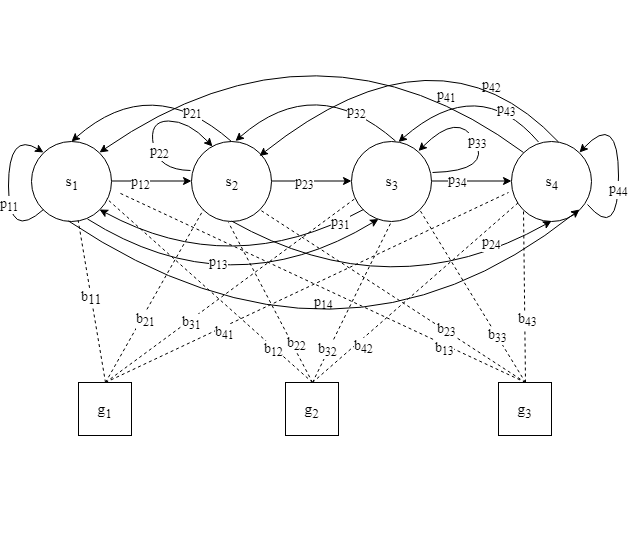
\includegraphics[width=0.5\textwidth]{ahmm.png}
    \caption{General Representation of an Adjusted Hidden Markov Model. In this image, states, emissions, and respective transition and emission probabilities are shown}
    \label{fig:hmm}
\end{figure}

\subsection{AHMM Based Prediction}
 Using the framework above, we build a model of a certain system offline. After $T$, the parameters of the AHMM can be used to make online predictions about the future states of the observed system. This is done by identifying the current state, $s_{i,T}$ and applying it to the transition and emission matrices, which are used as lookup tables, to obtain the next most likely state and its likelihood. We start with the assumption that $\mathcal{P}$ will give conclusive results
\begin{equation} \label{eq:nextstate}
    s_{i}(T+1) = \max_{j}[\mathcal{P}_{i(T),j}]
\end{equation}
There is, however, the possibility that there will be more than one returned states, as the maximum transition probability can be the same for multiple states. In this situation, we invoke the use of $\mathcal{B}$. Because the relationship between states and observations is not hidden, we can use the expected observation, derived from (\ref{eq:obsref}) to assess which returned state is more accurate. In the event that the prediction is still unclear, we elect the more dangerous transition, which is a quantity that depends on the application. For instance, in our case study, the more dangerous transition is one that minimizes the distance between our user's vehicle and the observed vehicle. In addition, we also update the model parameters online based on the actual observed transition, as will be described in the next section. Using this framework, it is possible to predict over any future horizon H, assuming that the prediction is correct at each iteration, the future states using the transition and emission matrices.

\begin{algorithm}[H]
\SetAlgoLined
\KwResult{$s(t+1)$}
 \While{$t\leq H$}{
  \For{$s(t) = s_i$}{
   $\max_j(\mathcal{P}_{ij})$, where $j = \{1,\ldots,n\}$
   }
   \eIf{$j$ is not a singleton}{
    $\forall j: \mathcal{B}_{jk}$, where $k =\{1,\ldots,m\}$\;
    }{
    $s_j = s(t+1)$\;
    }
    }
 \caption{Future State Prediction}
\end{algorithm}


\subsection{Online Updating and Training of AHMM Parameters}
AHMM parameters can be updated online in order to increase the accuracy of the model. This is done by using (\ref{eq:transbuild}) and (\ref{eq:obsbuild}) with another the new transition and associated observation. In addition, we use a sliding window approach such that $T$ always remains the same, such that
\begin{equation}
 T = t-T+t_l,t,\ldots,t+t_l    
\end{equation}
where $t$ represents the end of the training set, $T$ is the time horizon of the training set itself, and $t_l$ is the current time at which the window is being slid. If the system enters a new state or observation, $n$ or $m$ would increase, respectively. The updated parameters, $\mathcal{P'}$ and $\mathcal{B'}$, will continue to be used for online prediction.

\subsection{Online Model Fitting}
Using the framework described in Sections A,B, and C,  we can extract a model that captures the behavior of a system that we have been observing for $T$. Multiple models can be extracted using several data sets of different systems under observation. In other words, we can obtain super-sets containing all the transition and emission matrices.
\begin{equation}
    \hat{\mathcal{P}} = \{\mathcal{P},\ldots,\mathcal{P}_M\}
\end{equation}
\begin{equation}
    \hat{\mathcal{B}} = \{\mathcal{B},\ldots,\mathcal{B}_M\}
\end{equation}

During run-time we observe new measurements of other systems and the challenge becomes fitting each new system observations to the right model. However, until we have enough data about this new system, the prediction may not be correct, and thus, we need to take into account error, $\sigma$. In efforts to minimize situations where transitions are unclear, we propose training multiple models prior to the prediction process. With more models, we are more likely to find a precise fit. We use $M_1,M_2,\ldots,M_w$ to represent $w$ different models of some system. Using the method outlined in this section, we are able to determine and apply the best model.

Having built multiple models, we observe a new system and begin to execute the framework discussed in Section A for two measurements, $o(t-1),o(t)$. With this information, we are able to further execute the framework and determine parameters $\tilde{\mathcal{P}}$ and $\tilde{\mathcal{B}}$. In order to determine the optimal model, we calculate the errors between our model and each of the offline models:

\begin{equation} \label{probdist}
    \tilde{\sigma}_\mathcal{P} = \{\sigma_{\mathcal{P}_{1}},\ldots,\sigma_{\mathcal{P}_{w}}\} = \forall\mathcal{P}_w\in\hat{\mathcal{P}} \lVert \tilde{\mathcal{P}}-\hat{\mathcal{P}_w} \rVert
\end{equation}

%\begin{equation} \label{probdist}
    %\tilde{\sigma}_\mathcal{B} = %\{\sigma_{\mathcal{B}_{1}},\ldots,\sigma_{\mathcal{B}_{w}}\} = %\forall\mathcal{B}_w\in\hat{\mathcal{B}} \lVert %\tilde{\mathcal{B}}-\hat{\mathcal{B}_w} \rVert
%\end{equation}

In order to determine the model with the lowest error, we minimize the set $\tilde{\sigma}_\mathcal{P}$,

\begin{equation}
    w^* = \forall\sigma_{\mathcal{P}_w}\in\tilde{\sigma_\mathcal{P}}\text,  \min_{w} \tilde{\sigma_{\mathcal{P}_w}}
\end{equation}

The $M^*_{w}$ represents the model with the least error, or the optimal model. In order to make predictions using the optimal model, we use refer to the parameters, $\mathcal{P}_w$ and $\mathcal{B}_w$, where $w$ refers to the optimal model. The procedure to predict future states is as shown in *Algorithm*.



\subsection{Online Fitting for Uncertain Fits}
If the observed system, however, does not result in an $M^*_{w}$ with a high $\sigma$, the method outlined in the online section is used. Because we are attempting to fit the model, rather than build a new one, we have the advantage of having the baseline, the current $M^*_{w}$. We are able to leverage the parameters of $M^*_{w}$, by augmenting and updating $\tilde{\mathcal{P}}$ and $\tilde{\mathcal{B}}$ as we enter new states or observe new transitions or observations, much like how we obtain $\mathcal{P}'$ and $\mathcal{B}'$. With this, we obtain $\tilde{\mathcal{P}}'$ and $\tilde{\mathcal{B}}'$ In the case of a consistently diverging $\sigma$, we use $\tilde{\mathcal{P}}'$ and $\tilde{\mathcal{B}}'$ to make future predictions using *Algorithm*.

\section{Case Study: Semi-autonomous vehicle on a Highway}
In this section, we describe the case study we use to illustrate the use of the AHMM framework, and we demonstrate how it can be used to guarantee safe operation. The case study in this paper is that of a manned ground vehicle travelling in a typical highway setting.

\subsection{System Model}
The vehicle we use in our case study is a human-controlled vehicle with autonomous capabilities. The model used for the vehicle is that of a unicycle-type robot:
\begin{equation}
    \begin{cases}
    \dot{x} = u_s\cos{\theta} \\
    \dot{y} = u_s\sin{\theta} \\
    \dot{\theta} = u_\omega
    \end{cases}
\end{equation}
where $(x,y,\theta)$ is the robot position and orientation, and $(u_s,u_\omega)$ is the input control pair that represents linear and angular velocities. The inputs consist of autonomous and human controlled parts, $u_a$ and $u_h$. These values always satisfy the criteria $u_a+u_h = 1$. This vehicle will be known as the host vehicle, as it is where the computation takes place. In addition, all vehicles within a certain sensing range of the host vehicle are modeled as follows:
\begin{equation} \label{eq:agentpos}
    \forall q \in R:
    \begin{cases}
    \dot{x}_q = v_q \\
    \dot{y}_q = v_q\ \\
    \theta_q = l
    \end{cases}
\end{equation}
where $q$ represents each vehicle in sensing range $R$, and $l$ represents the lane that the vehicle is in. These vehicles will be known as agents.

\subsection{Environment Setup}
The highway environment, which we are studying, involves three lanes with multiple vehicles, that can change their velocities and their lanes. Within the highway environment, we are able to set up two AHMMs to capture the behaviors we expect to see. The AHMMs are applied to all of the agents.

The first AHMM will aim to predict future velocities of the agents. In this model,

\begin{equation}
\{s_1,s_2,\ldots s_n\} = \{v_1,\ldots v_n\}
\end{equation}
    where $v$ represents velocity. The emissions reflect the relationship between $v_{t+1}$ and $v_t$:

\begin{enumerate}
    \item Speeding Up, where $v_{t+1} > v_t$
    \item Slowing Down, where $v_{t+1} < v_t$
    \item Maintaining Speed, where $v_{t+1} \approx v_t$
\end{enumerate}

The second AHMM will be used to predict the lateral position of the agents. The positions, for our purposes, are modeled as discreet lanes: (Left, Center, Right);

\begin{equation}
    \mathbf{L} = \{L,C,R\}
\end{equation}

In this model, states represent distances between preceding agents:

\begin{equation}
\{s_1,s_2,\ldots s_n\} = \{d_1,\ldots d_n\}
\end{equation}

where $d$ represents the distance between the relevant agent, $q$, and a preceding agent its lane. The emissions reflect reactions to the preceding agent and are as follows:
\begin{enumerate}
    \item Changing Left
    \item Changing Right
    \item Not Changing
\end{enumerate}
In this case, the relationship between states and emissions indicates at what distance $d_n$ we can expect the agent to react to the preceding agent.

Multiple models can be trained using the AHMM framework, yielding $\mathcal{P}$ and $\mathcal{B}$ matrices for each model, and these models can be used for fitting, updating, augmentation, and most importantly, prediction, as discussed in the previous sections. Using the method for fitting models, we are able to identify $M^*$ from a set of pretrained models, which consists of the appropriate AHMM parameters for the optimal model, for both velocity and lateral position.

\subsection{Using AHMM Method for Safe Vehicle Operation}
Using the optimal model for each agent, we are able to predict where an agent will be in the environment for a certain user-defined time horizon, $T_{u}$. This time horizon defines how far ahead the user wants the system to calculate the appropriate action to take.  A sequence of future states for agent $q$, both in terms of velocity and lateral position, are developed using the AHMM parameters. Given a sequence of future expected velocities, we are able to calculate the forward positions for the user-defined forward positions using:

\begin{equation} \label{eq:dumpos}
    y(t) = v_qt
\end{equation}

where $t$ represents a time within $T_{u}$. The AHMM for lateral position tells us what type of lane change action to expect as we observe a certain $d$ between agents. Using this information, we build a risk profile and adapt the host vehicle's input accordingly.


\subsubsection{Risk Estimation based on Online Prediction}
This section shows how risk is defined given our online prediction over $T_{u}$. Risk is always connected to the host vehicle's actions. For example, if the user is driving the vehicle at a certain velocity $u_s$ with no indication of turning, $u_\omega = \pi/2$, we assume that action will continue for the length of $T_{u}$ and a lane change will not occur, and we calculate future forward positions using (\ref{eq:dumpos}). With this, we can estimate the future positions of the host vehicle. In addition, risk will be calculated as a separate entity for each lane, $l$.

The risk is a function of the distance between estimated future positions of the host vehicle and the agents at each $t$ within time horizon $T_{u}$. The distance is calculated using the following equation:

\begin{equation}
    \forall q \in R : d_q = y_t - y_{q}(t)
\end{equation}

where the subscript $q$ indicates a particular agent, and is evaluated for all $t \leq T_u$. The choice to make this distance a simple difference, rather than euclidean or absolute distance was made in order to is the sign to accurately capture the direction of the source of the risk; whether it is coming from in front of or behind our vehicle. We will use $r$ to denote this risk, which increases as distance decreases. The following equation demonstrates how we calculate risk:

\begin{equation}
    r_{q}^{f}(t) =
    \begin{cases}
    1,                      & \text{if } d_{q}(t) < 1 \\
    \frac{1}{d_{q}(t)},  & \text{otherwise} 
    \end{cases}
\end{equation}

where $r_{q}^{l}(t)$ represents the risk of a certain agent $q$ interfering with the user's position in a certain lane $l$ at time $t \leq T_u$. It is important to note that multiple agents affect risk in our analysis, the agent with the highest absolute risk is considered for adaptation. The set of maximum risk values for each lane is evaluated for each $t \leq T_u$:

\begin{equation}
    \hat{\mathcal{R}} = \{\hat{r}^{L},\hat{r}^{C},\hat{r}^{R}\}
\end{equation}

\subsubsection{Adaptive User Assistance}
Given the $\hat{r}$ values for each lane for all $t \leq T_u$, we can adapt our system to guarantee safety. In order to adapt to the user's actions, we need to first identify whether these actions are going to result in a dangerous situation. A user parameter, $\rho$ is used as a threshold for risk. This value must satisfy the condition: $0<\rho<1$. A high $\rho$ would indicate that the user is willing to incur more risk, while a lower $\rho$ would indicate a more conservative driver. Given this value, our system does not interfere with the actions of the vehicle unless the maximum risk in the user's lane surpasses $\rho$, as is shown below:

\begin{equation}
    u_a > u_h \iff \hat r^{l_u} > b
\end{equation}

where $u_a$ and $u_h$ represent autonomous and human inputs, while $l_u$ represents the user's lane and $l_u \in \mathbb{L}$. In the case that the autonomous control input surpasses that of the user input, the system analyzes the correct action to take. Because the risk is calculated for each lane, the initial action is to identify if a certain lane has a lower risk. With this, we identify $l^*$, which is the lane with the lowest risk:

\begin{equation}
    l^* = \min_l(\mathcal{R})
\end{equation}

In addition, we determine the minimum and maximum velocities our vehicle should be driving within one lane. These values are calculated as follows:

\begin{equation}
    v_min = d_{q,min}/T_u
\end{equation}

\begin{equation}
    v_max = d_{q,\min}/T_u
\end{equation}

 Let us take, for example, our host vehicle travelling at a much higher velocity than a preceding agent in the same lane. Our system identifies that our user has not shown any sign of turning, and because of that, we assume the user's priority is to stay in the lane. As a result of this, the $u_a$ involves lowering the velocity first. Assuming that the user doesn't respond, our system will continue to lower the velocity such that $u_s = v_q$, as long as the risk remains below $\rho$. If the user respond with a sub-optimal lane change, then the system will assist the user by reverting to the optimal action instead.  


\section{Simulations}
The simulations for this work primarily were done in Matlab. Different simulations were run for each part of the approach and case study shown above. We first discuss how the models were trained, and we validate those results for both velocity and lateral positions. This is followed by showing an example of fitting one model given multiple pre-trained models and a new system to observe. Lastly we demonstrate the risk estimates, and the adjustments made to user actions, in order to verify that we are able to guarantee safety.

\subsection{Training Models}
For training the models, we used a workspace featuring $15$ stationary obstacles. A test vehicle drove through a highway setting with these obstacles, and it was observed for a training period of 700 iterations. This is followed by an estimation period of 700 iterations, which were used to validate the parameters.

\begin{figure}[ht]
    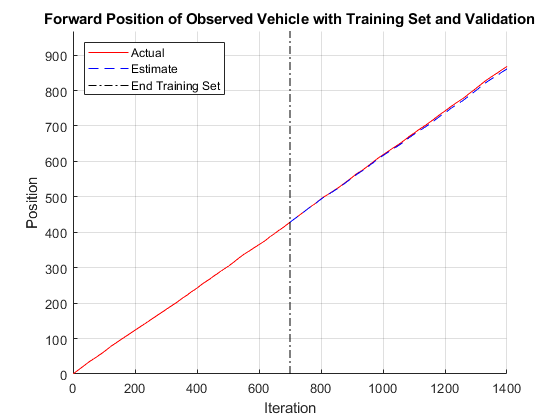
\includegraphics[width=0.5\textwidth]{train1.png}
    \caption{The forward position of the actual robot (red) is shown. After the training set, a prediction is made and the forward position of the estimate is shown (blue dashed).}
    \label{fig:cs1}
\end{figure}

\begin{figure}[ht]
    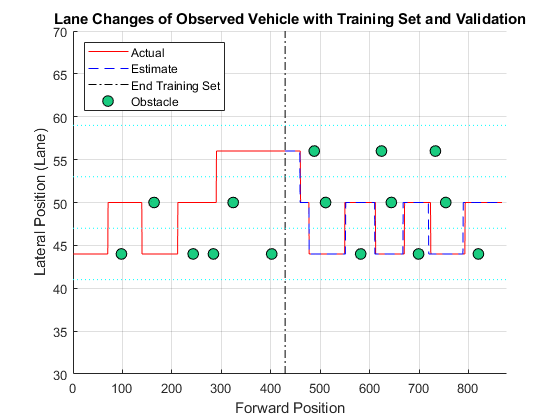
\includegraphics[width=0.5\textwidth]{train2.png}
    \caption{The lane changes of the actual robot (red) are shown. After the training set, a prediction is made and the lateral positions/lane changes of the estimate is shown (blue dashed).}
    \label{fig:cs1b}
\end{figure}

In this simulation we find that the root mean squared error (RMSE) between the forward positions is $3.9273$, and the RMSE between lane changes is $2.5912$.  

\subsection{Fitting Models}

In the next simulation, we show that we are able to fit pre-trained models to a certain vehicle, whose behaviors are randomly generated, moving through the same workspace as the training sets. In this simulation, we begun to fit the parameters after making one full transition and obtaining related emissions. 

\begin{figure}[ht]
    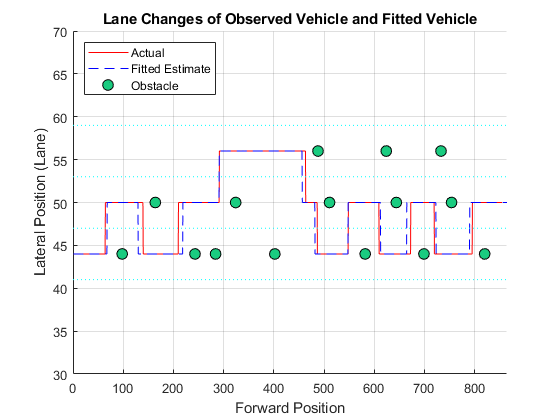
\includegraphics[width=0.5\textwidth]{fit2.png}
    \caption{The forward position of the actual robot (red) is shown. In addition, the forward position of the best-fit is shown (blue dashed).}
    \label{fig:cs1}
\end{figure}

\begin{figure}[ht]
    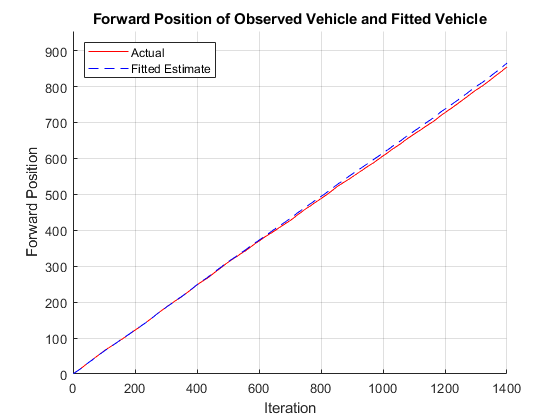
\includegraphics[width=0.5\textwidth]{fit1.png}
    \caption{The lane changes of the actual robot (red) are shown. The lane change predictions of the best-fit are shown (blue dashed).}
    \label{fig:cs1b}
\end{figure}
 In addition, we show the error of the fit for each velocity model in \ref{fig:cs1c}.
 
 \begin{figure}[ht]
    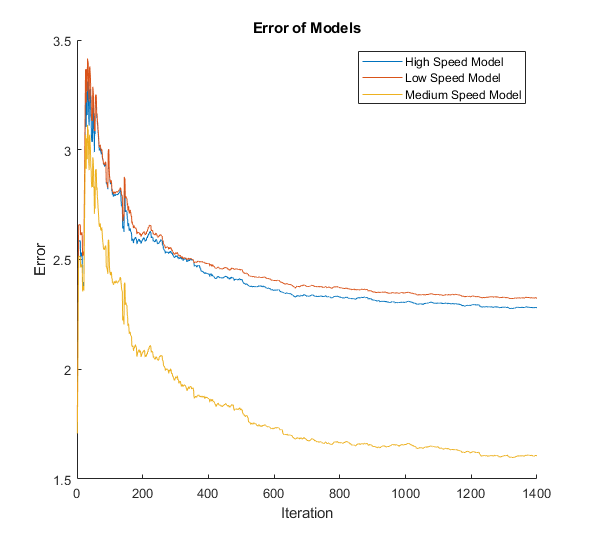
\includegraphics[width=0.5\textwidth]{fit3.png}
    \caption{The error of the fit between our model and each of the three pretrained models}
    \label{fig:cs1c}
\end{figure}

Here we see that the closest fit is that of the medium-speed model.
 
 
\subsection{Avoidance}
In order to show the proactive safety system, we have three specific use-cases.

In the first case, the host vehicle in the center lane responds to the actions and future position of a vehicle in the left lane, which is passing a stationary obstacle. The two snapshots of the simulation in Fig.\ref{fig:cs1} and Fig.\ref{fig:cs1b} indicate the behaviors that are occurring.

\begin{figure}[ht]
    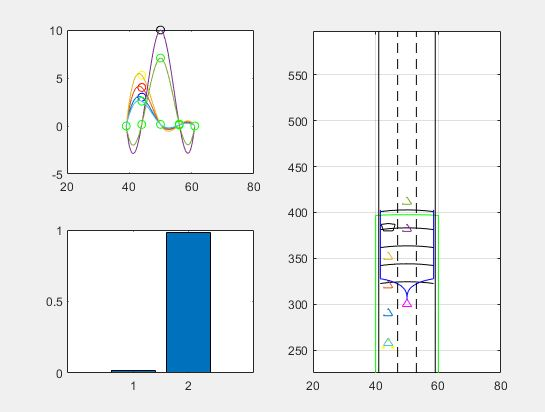
\includegraphics[width=0.5\textwidth]{cs1.JPG}
    \caption{In this snapshot, $u_{\alpha} = 0$ and $u_{h} = 1$. This is because the $r^l$ at $T_u$ is below the $\rho$.}
    \label{fig:cs1}
\end{figure}

\begin{figure}[ht]
    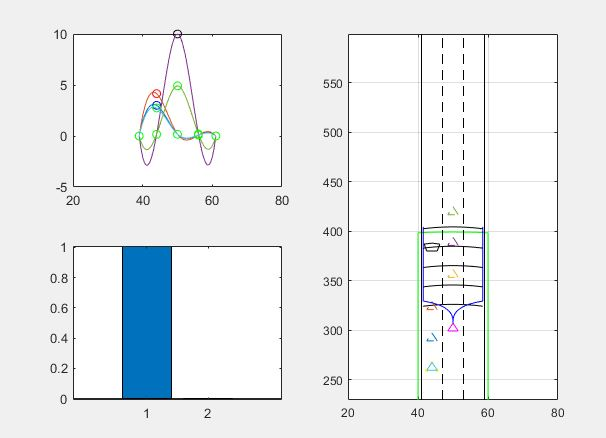
\includegraphics[width=0.5\textwidth]{cs1b.JPG}
    \caption{In this snapshot, the risk in the host vehicle's lane at $T_u$ has increased above $\rho$, and autonomy has increased rapidly. The reason $u_{alpha}$ has increased to 1, is because this is the instant at which the change begins. The location of minimum risk is determined to be the right lane, and the vehicle will then move to the right lane.}
    \label{fig:cs1b}
\end{figure}

This simulation results in a safe operation, as the minimum risk is easily identified and the solution is offered. In this simulation, the human takes no action, which is another reason fully autonomous intervention occurs, and the risk is still minimized and avoided.


In the second simulation, the human does take some action and it is evident that autonomy and human-control are fluid and change based on changing surroundings. In addition, there is once again a clear location at which the risk is at a minimum. The snapshot in Fig.\ref{fig:cs2} shows a situation where the user is travelling at a velocity slightly too rapid for the obstacle ahead, and slowing down will not put it at a risky position in relation to the next vehicle that is behind the user. As a result, $u_{\alpha}$ is increased as the level of risk increases.

\begin{figure}[ht]
    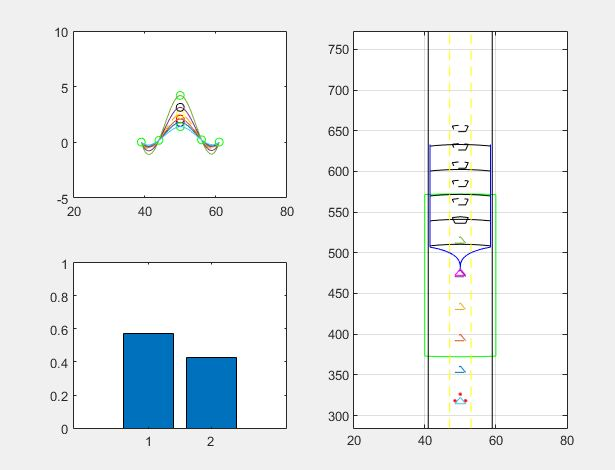
\includegraphics[width=0.5\textwidth]{cs2.JPG}
    \caption{In this snapshot, $u_{\alpha} > u_{h}$. This is because the $r^l_u$ at $T_u$ is above $\rho$}
    \label{fig:cs2}
\end{figure}

This result also indicates a case of the user's desires being met as closely as possible. The user, by only adjusting velocity and not adjusting their lane change behavior, indicates that the velocity is the first parameter to adjust. As shown in Fig.\ref{fig:cs2c}, the velocity is only adjusted so that the driver is in a safe position for the selected time $T_u$ and, consequently for times $t,t+1,\ldots,T_u$. This is indicated by a velocity that slowly decreases to a safe value. This, however, would only suffice to maximize the time before a collision occurs. Because that is a limitation of only adjusting the velocity, when a collision becomes imminent, $u_\alpha$ increases to 1, and the lane is changed to that of minimum risk.

\begin{figure}[ht]
    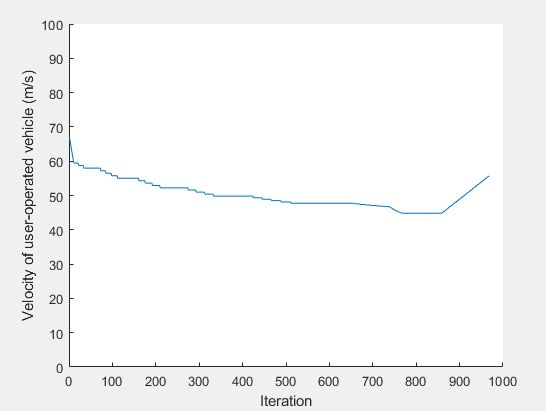
\includegraphics[width=0.5\textwidth]{cs2c.JPG}
    \caption{This figure depicts the velocity of the user's vehicle}
    \label{fig:cs2c}
\end{figure}

The third case is built much like the second case. In this implementation, however, neither of the two surrounding lanes are available. In this case, the system begins to react much like that of the second case, however, there is a error in the prediction of what the following vehicle will do. This is because the model was trained for a lane change, but it is evident that a lane change will not occur when the actual vehicle (not the estimates) approaches our user's vehicle. An adjustment of the velocities in this case are shown in \ref{fig:vehiclepos}. In a situation like this, the algorithm does delay the imminent collision, but there is a specific preference to retain a certain following distance, $d_q$ behind the obstacle in front. We assume that the user's vehicle has a responsibility to not directly cause a collision on its own. This does, however, leave the possibility of a rear collision, which is addressed further in the discussion.


\section{Experiment}
\section{Conclusions}

\newpage
% references section

% can use a bibliography generated by BibTeX as a .bbl file
% BibTeX documentation can be easily obtained at:
% http://mirror.ctan.org/biblio/bibtex/contrib/doc/
% The IEEEtran BibTeX style support page is at:
% http://www.michaelshell.org/tex/ieeetran/bibtex/
%\bibliographystyle{IEEEtran}
% argument is your BibTeX string definitions and bibliography database(s)
%\bibliography{IEEEabrv,../bib/paper}
%
% <OR> manually copy in the resultant .bbl file
% set second argument of \begin to the number of references
% (used to reserve space for the reference number labels box)

%\begin{thebibliography}{1}

%\bibitem{IEEEhowto:kopka}
%H.~Kopka and P.~W. Daly, \emph{A Guide to \LaTeX}, 3rd~ed.\hskip 1em %plus
%  0.5em minus 0.4em\relax Harlow, England: Addison-Wesley, 1999.
  
  
%\end{thebibliography}

%\printbibliography
\bibliographystyle{abbrv}
\bibliography{mybibliography.bib}


% that's all folks
\end{document}


